% ==============================================================================
% VLIZ Scientific Research Poster - LOD Docker Webserver (Option 1 Top-Hero Flow)
% ==============================================================================
% Audience: Interdisciplinary Data Stewards & Open Science Practitioners
% Layout: Option 1 — Top Hero Showcase + Multi-Column Chronological Flow
% Branding: VLIZ Sea-Teal (#91C8CD) + Corporate Navy (#3057A5)
% Empirical Standard: Khadka & Peeters (2024) MAR Exemplary Tier (70/30 Rule)
% ==============================================================================

\documentclass[
  25pt,
  a0paper,
  portrait,
  margin=0mm,
  innermargin=15mm,
  blockverticalspace=7mm,
  colspace=10mm,
  subcolspace=8mm
]{tikzposter}

\usepackage{graphicx}
\graphicspath{{assets/}{posters/lod-docker-webserver/assets/}{templates/posters/assets/}}
\usepackage{amsmath,amssymb}
\usepackage{qrcode}
\usepackage{hyperref}
\usepackage{tikz}
\usetikzlibrary{positioning,calc,arrows.meta}
\usepackage{tcolorbox}

% ------------------------------------------------------------------------------
% VLIZ Institutional Color Palette
% ------------------------------------------------------------------------------
\definecolor{vlizBanner}{HTML}{91C8CD}       % Sea-teal top banner
\definecolor{vlizTeal}{HTML}{31B7BC}         % Vibrant teal subtitle & accents
\definecolor{vlizNavy}{HTML}{3057A5}         % VLIZ Corporate Navy
\definecolor{vlizCharcoal}{HTML}{231F20}     % Dark Charcoal author text
\definecolor{vlizSlateText}{HTML}{1E293B}    % Main body text
\definecolor{vlizSlateMuted}{HTML}{64748B}   % Muted caption/affiliation text
\definecolor{vlizCardBg}{HTML}{FFFFFF}       % White card background
\definecolor{vlizHeroBg}{HTML}{F8FAFC}       % Soft slate sub-card background
\definecolor{vlizBorder}{HTML}{CBD5E1}       % Card border
\definecolor{vlizLightTeal}{HTML}{E6F7F8}   % Light teal callout background

% Set custom tikzposter style
\definecolorstyle{VLIZStyle}{
  \definecolor{colorOne}{HTML}{3057A5}
  \definecolor{colorTwo}{HTML}{31B7BC}
  \definecolor{colorThree}{HTML}{91C8CD}
}{
  \colorlet{backgroundcolor}{white}
  \colorlet{framecolor}{white}
  \colorlet{titlefgcolor}{vlizNavy}
  \colorlet{titlebgcolor}{white}
  \colorlet{blocktitlebgcolor}{white}
  \colorlet{blocktitlefgcolor}{vlizNavy}
  \colorlet{blockbodybgcolor}{vlizCardBg}
  \colorlet{blockbodyfgcolor}{vlizSlateText}
}

\usetheme{Default}
\usecolorstyle{VLIZStyle}
\tikzposterlatexaffectionproofoff

% Custom block style: Clean rounded card with crisp border
\defineblockstyle{VLIZBlock}{
  titlewidthscale=1.0, bodywidthscale=1.0,
  titleoffsetx=0pt, titleoffsety=0pt, bodyoffsetx=0pt, bodyoffsety=0pt,
  bodyverticalshift=0pt, roundedcorners=14, linewidth=2pt,
  titleinnersep=4mm, bodyinnersep=5.5mm
}{
  \draw[color=vlizBorder, fill=blockbodybgcolor, rounded corners=14, line width=2pt]
    (blockbody.south west) rectangle (blocktitle.north east);
}
\useblockstyle{VLIZBlock}

\title{}
\author{}
\institute{}

\begin{document}

% ==============================================================================
% 1. TOP BANNER (Official VLIZ Vector Header)
% ==============================================================================
\fill[vlizBanner] (-0.5\paperwidth, 0.5\paperheight)
  rectangle (0.5\paperwidth, {0.5\paperheight - 0.112\paperheight});

% Vector VLIZ Logo (Left)
\node[anchor=west, inner sep=0pt] at ({-0.5\paperwidth + 0.088\paperwidth}, {0.5\paperheight - 0.056\paperheight}) {
  
\includegraphics[height=0.064\paperheight]{vliz_logo.png}
};

% Native Vector Typography for URL (Right)
\node[anchor=east, inner sep=0pt] at ({0.5\paperwidth - 0.088\paperwidth}, {0.5\paperheight - 0.056\paperheight}) {
  {\color{vlizNavy}\sffamily\bfseries\fontsize{34pt}{40pt}\selectfont vliz.be}
};

% ==============================================================================
% 2. TITLE & AUTHORS SECTION
% ==============================================================================
\node[anchor=north west, text width=0.88\paperwidth, align=flush left, inner sep=0pt]
  at ({-0.5\paperwidth + 0.06\paperwidth}, {0.5\paperheight - 0.122\paperheight}) {
  % Subtitle / Topic Callout
  {\color{vlizTeal}\bfseries\Large OPEN SCIENCE \& WEB ARCHITECTURE \quad $\vert$ \quad 30 DISCOVERY CHANNELS \quad $\vert$ \quad DOCKER TESTBED \par}
  \vspace{0.22cm}
  % Main Title
  {\color{vlizNavy}\bfseries\fontsize{38pt}{46pt}\selectfont LOD Docker Webserver: A Multi-Channel Testbed for Linked Data Discovery \par}
  \vspace{0.24cm}
  % Author Attribution
  {\color{vlizCharcoal}\large \underline{\textbf{Cedric Decruw}}$^{*,1}$ \par}
  \vspace{0.12cm}
  % Affiliations & Contact
  {\color{vlizSlateMuted}\normalsize $^1$Flanders Marine Institute (VLIZ), InnovOcean Campus, Ostend, Belgium \quad $\vert$ \quad $^*$Corresponding Author: cedric.decruw@vliz.be \par}
};

% ==============================================================================
% Set starting vertical position for tikzposter blocks
% ==============================================================================
\makeatletter
\setlength{\TP@blocktop}{0.5\textheight - 250mm}
\makeatother

% ==============================================================================
% 3. HERO INFOGRAPHIC SHOWCASE (Top Banner Zone, 42% Canvas Height)
% ==============================================================================
\block{}{
  \centering
  \vspace{-0.15cm}
  {\color{vlizNavy}\bfseries\huge Multi-Channel Testbed Architecture \& 2$\times$2 Discovery Taxonomy \par}
  \vspace{0.14cm}
  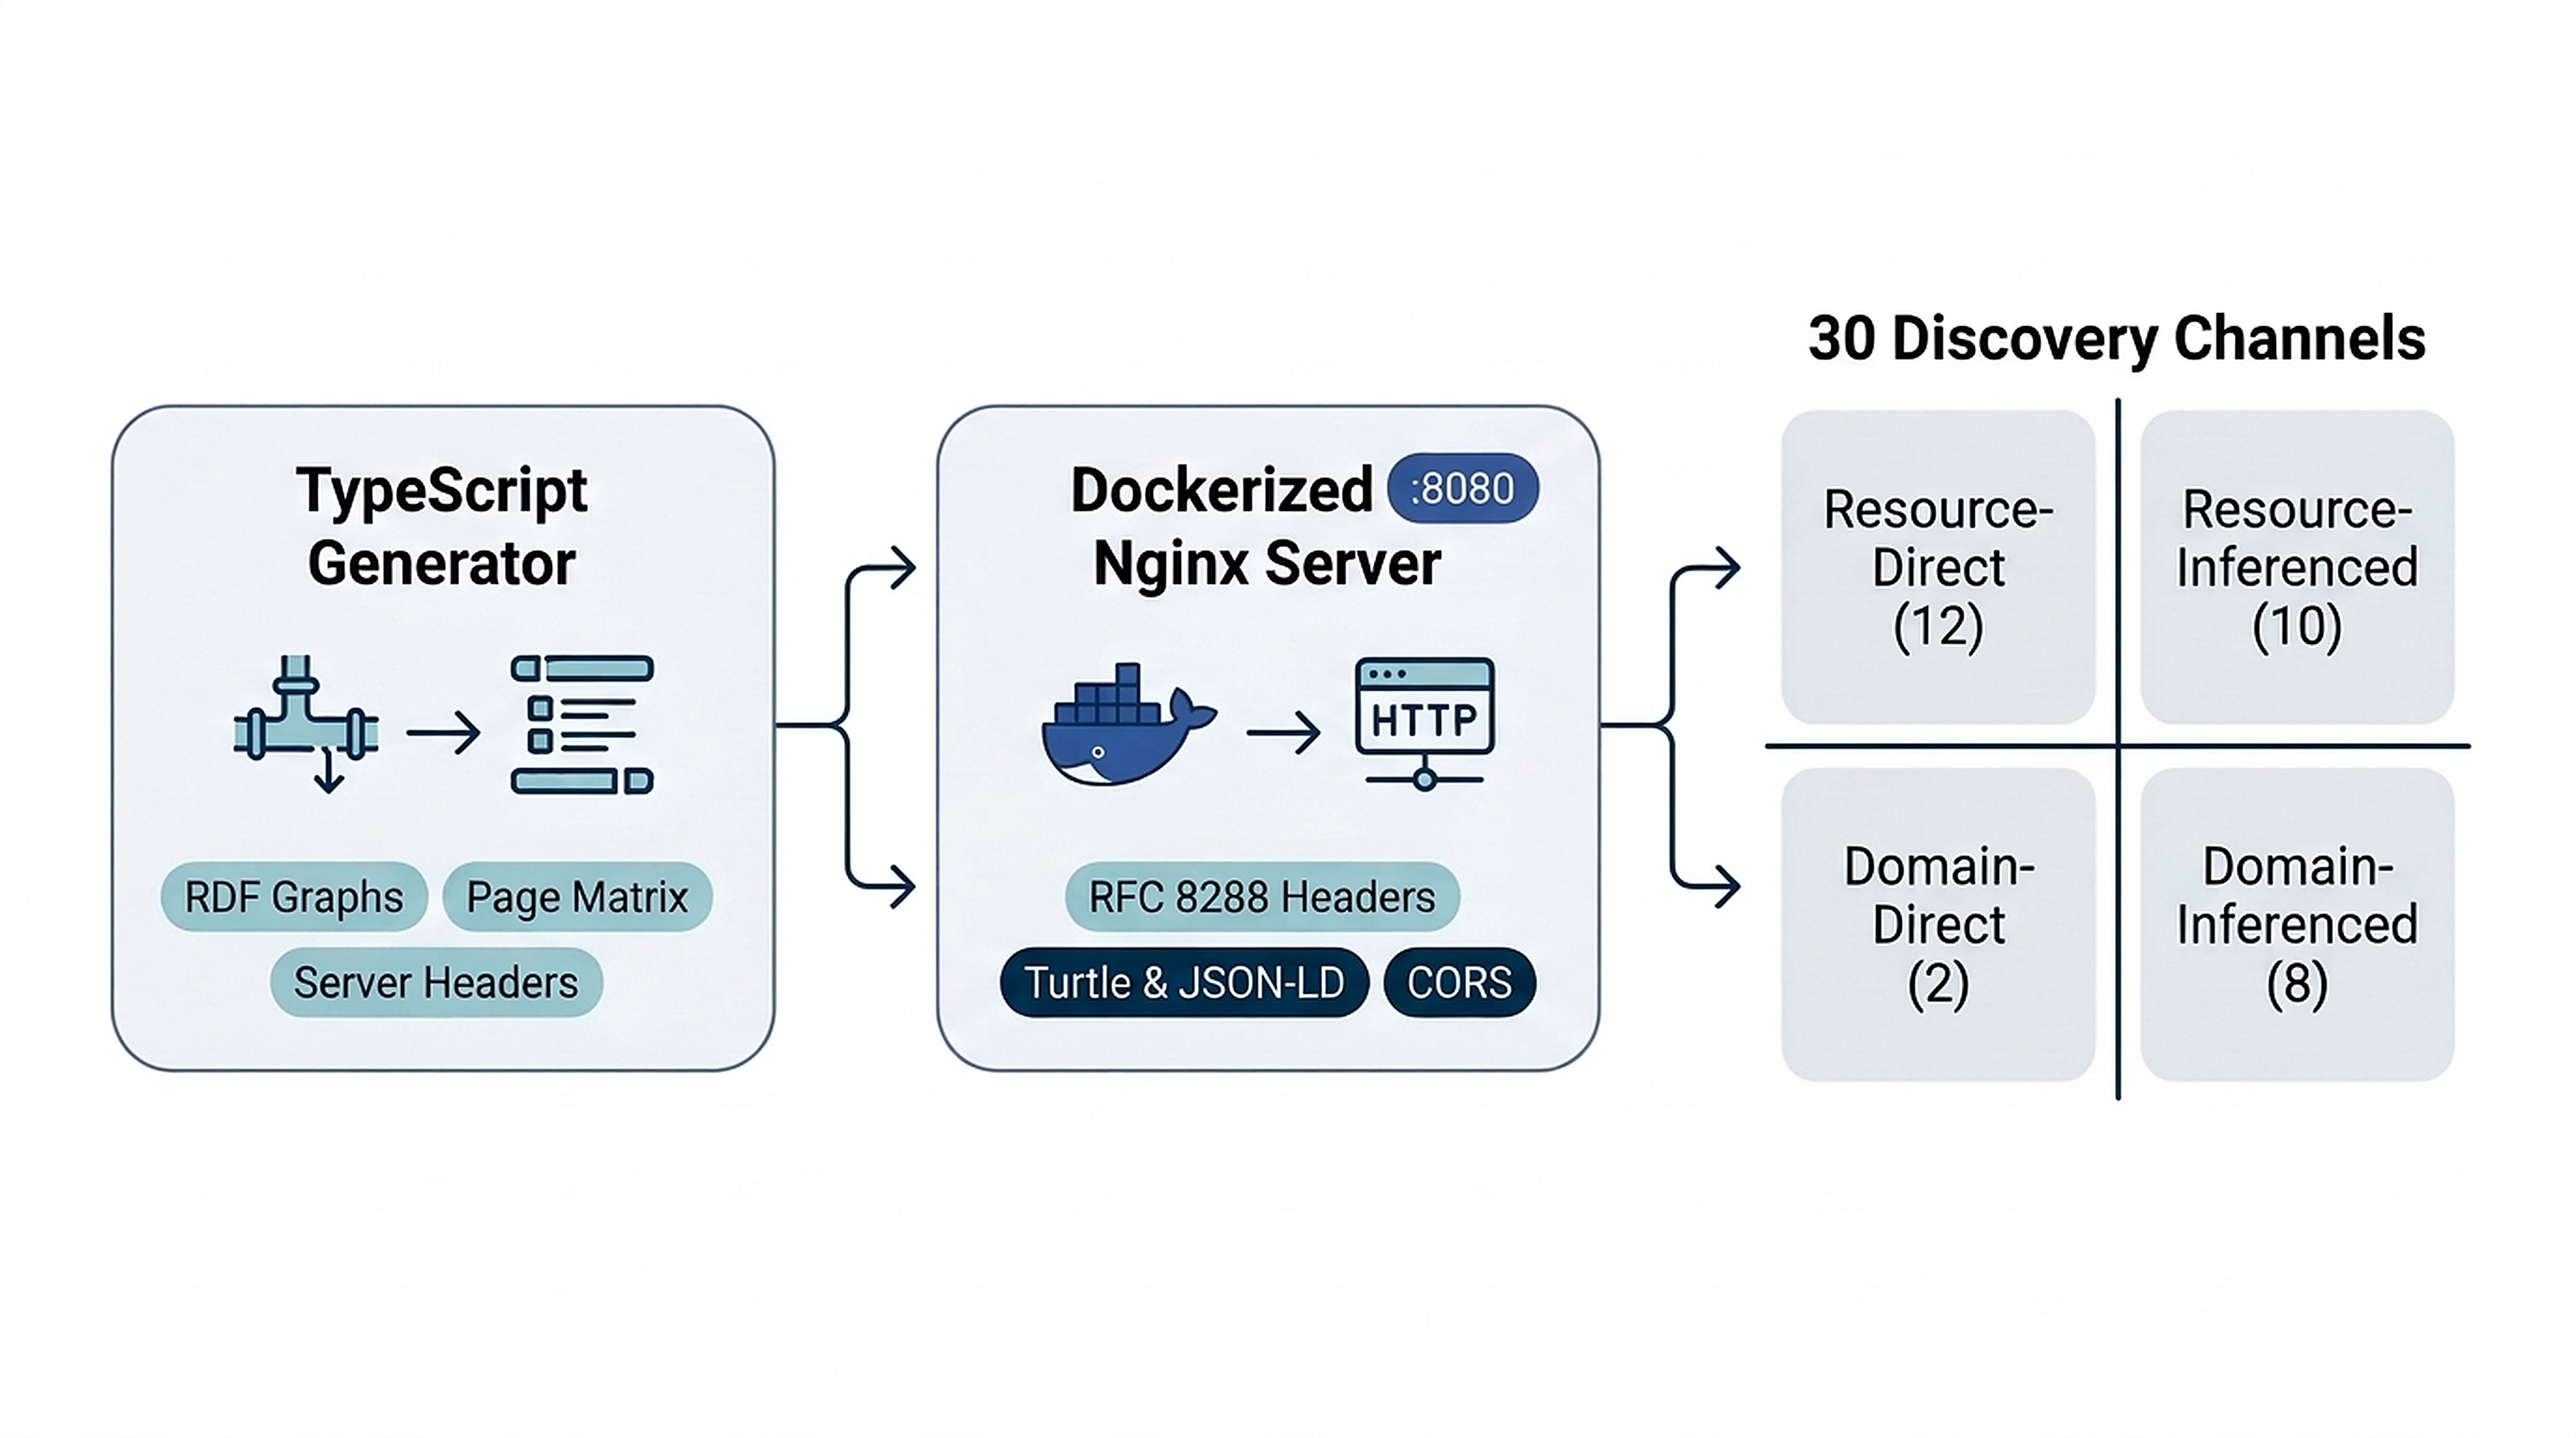
\includegraphics[width=0.96\linewidth]{hero_infographic_hd.png}\\[-0.02cm]
  {\color{vlizSlateMuted}\normalsize \textbf{Figure 1:} Multi-channel LOD testbed architecture uniting TypeScript generator, containerized Nginx, and 30-channel taxonomy.}
  \vspace{-0.1cm}
}

% ==============================================================================
% 4. BALANCED 2-COLUMN NARRATIVE (Below Hero Infographic)
% ==============================================================================
\begin{columns}
  % ----------------------------------------------------------------------------
  % LEFT COLUMN: Context & Formulation -> Empirical Discovery Metrics
  % ----------------------------------------------------------------------------
  \column{0.50}

  % Section 1: Context & Core Problem (Styled Mini-Cards)
  \block{1. Context \& Problem Formulation}{
    \noindent
    \begin{minipage}{0.315\linewidth}
      \begin{tcolorbox}[colback=vlizLightTeal,colframe=vlizBanner,arc=3.5mm,boxrule=1.4pt,left=3.5mm,right=3.5mm,top=2.2mm,bottom=2.2mm,height=4.8cm]
        {\color{vlizNavy}\bfseries Discovery Gap}\\[2pt]
        {\footnotesize Linked Data fails when machines must guess where RDF graphs and relation types are exposed [1].}
      \end{tcolorbox}
    \end{minipage}\hfill
    \begin{minipage}{0.315\linewidth}
      \begin{tcolorbox}[colback=vlizLightTeal,colframe=vlizBanner,arc=3.5mm,boxrule=1.4pt,left=3.5mm,right=3.5mm,top=2.2mm,bottom=2.2mm,height=4.8cm]
        {\color{vlizNavy}\bfseries Crawler Fragility}\\[2pt]
        {\footnotesize Harvesters rely on brittle heuristics and domain guessing rather than formal RFC signposts [2].}
      \end{tcolorbox}
    \end{minipage}\hfill
    \begin{minipage}{0.315\linewidth}
      \begin{tcolorbox}[colback=vlizLightTeal,colframe=vlizBanner,arc=3.5mm,boxrule=1.4pt,left=3.5mm,right=3.5mm,top=2.2mm,bottom=2.2mm,height=4.8cm]
        {\color{vlizNavy}\bfseries Zero Benchmarks}\\[2pt]
        {\footnotesize No unified testbed previously isolated and cross-evaluated channels under controlled semantics [3].}
      \end{tcolorbox}
    \end{minipage}

    \vspace{0.16cm}
    \begin{tcolorbox}[colback=vlizHeroBg,colframe=vlizBorder,arc=4mm,boxrule=1.5pt,left=5mm,right=5mm,top=2.6mm,bottom=2.6mm]
      {\color{vlizNavy}\bfseries Research Question (RQ)}\\[2pt]
      {\small\textit{How can containerized server semantics and multi-channel signposting be unified into an inspectable testbed to systematically evaluate Linked Data discovery across resource and domain tiers?}}
    \end{tcolorbox}

    \vspace{0.14cm}
    \begin{tcolorbox}[colback=vlizLightTeal,colframe=vlizTeal,arc=4mm,boxrule=1.5pt,left=5mm,right=5mm,top=2.6mm,bottom=2.6mm]
      {\color{vlizNavy}\bfseries Hypothesis \& Prediction}\\[2pt]
      {\small\textit{A dual-axis matrix (Location: Resource vs. Domain; Extraction: Direct vs. Inferenced RDF) deployed in an Nginx Docker testbed provides deterministic benchmarking across all 30 discovery channels.}}
    \end{tcolorbox}
    \vspace*{1.5mm}
  }

  % Section 3: Empirical Discovery Metrics (Verifiable Badges & Findings)
  \block{3. Empirical Discovery Metrics}{
    \noindent
    \begin{minipage}{0.235\linewidth}
      \begin{tcolorbox}[colback=vlizLightTeal,colframe=vlizNavy,arc=3.5mm,boxrule=1.8pt,halign=center,top=2.2mm,bottom=2.2mm]
        {\color{vlizNavy}\bfseries\fontsize{24pt}{28pt}\selectfont 30}\\[2pt]
        {\footnotesize\textbf{Channels Classified}}
      \end{tcolorbox}
    \end{minipage}\hfill
    \begin{minipage}{0.235\linewidth}
      \begin{tcolorbox}[colback=vlizHeroBg,colframe=vlizTeal,arc=3.5mm,boxrule=1.8pt,halign=center,top=2.2mm,bottom=2.2mm]
        {\color{vlizTeal}\bfseries\fontsize{24pt}{28pt}\selectfont 4}\\[2pt]
        {\footnotesize\textbf{Discovery Quadrants}}
      \end{tcolorbox}
    \end{minipage}\hfill
    \begin{minipage}{0.235\linewidth}
      \begin{tcolorbox}[colback=vlizLightTeal,colframe=vlizNavy,arc=3.5mm,boxrule=1.8pt,halign=center,top=2.2mm,bottom=2.2mm]
        {\color{vlizNavy}\bfseries\fontsize{24pt}{28pt}\selectfont 150}\\[2pt]
        {\footnotesize\textbf{Synthetic Pages}}
      \end{tcolorbox}
    \end{minipage}\hfill
    \begin{minipage}{0.235\linewidth}
      \begin{tcolorbox}[colback=vlizHeroBg,colframe=vlizTeal,arc=3.5mm,boxrule=1.8pt,halign=center,top=2.2mm,bottom=2.2mm]
        {\color{vlizTeal}\bfseries\fontsize{24pt}{28pt}\selectfont 100\%}\\[2pt]
        {\footnotesize\textbf{Deterministic Stack}}
      \end{tcolorbox}
    \end{minipage}

    \vspace{0.16cm}
    \begin{tcolorbox}[colback=vlizHeroBg,colframe=vlizBorder,arc=4mm,boxrule=1.5pt,left=5mm,right=5mm,top=2.8mm,bottom=2.8mm]
      {\color{vlizNavy}\bfseries Verifiable Multi-Channel Discovery}\\[2pt]
      {\small The testbed confirms that direct RDF channels provide high-confidence semantic acquisition without heuristic parsing, while inferenced channels supply essential catalog discovery and fallback harvesting across domain roots.}
    \end{tcolorbox}
    \vspace*{2.0mm}
  }

  % ----------------------------------------------------------------------------
  % RIGHT COLUMN: The 4 Strategic Pillars -> Discussion & Digital Access
  % ----------------------------------------------------------------------------
  \column{0.50}

  % Section 2: The 4 Strategic Pillars (2x2 Matrix)
  \block{2. The 4 Strategic Pillars}{
    \noindent
    \begin{minipage}{0.488\linewidth}
      \begin{tcolorbox}[colback=vlizLightTeal,colframe=vlizBanner,arc=3.5mm,boxrule=1.4pt,left=4mm,right=4mm,top=2.2mm,bottom=2.2mm,height=4.8cm]
        {\color{vlizNavy}\bfseries 1. Generator Pipeline}\\[2pt]
        {\footnotesize Staged TypeScript build compiling 150 synthetic pages with alternate RDF serializations.}
      \end{tcolorbox}
    \end{minipage}\hfill
    \begin{minipage}{0.488\linewidth}
      \begin{tcolorbox}[colback=vlizLightTeal,colframe=vlizBanner,arc=3.5mm,boxrule=1.4pt,left=4mm,right=4mm,top=2.2mm,bottom=2.2mm,height=4.8cm]
        {\color{vlizNavy}\bfseries 2. Container Delivery}\\[2pt]
        {\footnotesize Minimal Dockerized Nginx stack on port 8080 exposing explicit CORS, MIME, and Link headers.}
      \end{tcolorbox}
    \end{minipage}

    \vspace{0.14cm}
    \noindent
    \begin{minipage}{0.488\linewidth}
      \begin{tcolorbox}[colback=vlizHeroBg,colframe=vlizBorder,arc=3.5mm,boxrule=1.4pt,left=4mm,right=4mm,top=2.2mm,bottom=2.2mm,height=4.8cm]
        {\color{vlizNavy}\bfseries 3. Dual-Axis Taxonomy}\\[2pt]
        {\footnotesize 2$\times$2 matrix categorizing 30 channels across Location (Resource/Domain) and Extraction.}
      \end{tcolorbox}
    \end{minipage}\hfill
    \begin{minipage}{0.488\linewidth}
      \begin{tcolorbox}[colback=vlizHeroBg,colframe=vlizBorder,arc=3.5mm,boxrule=1.4pt,left=4mm,right=4mm,top=2.2mm,bottom=2.2mm,height=4.8cm]
        {\color{vlizNavy}\bfseries 4. Topology Validation}\\[2pt]
        {\footnotesize Complex graph simulations evaluating cyclic loops, pagination, and reciprocal backlinks.}
      \end{tcolorbox}
    \end{minipage}

    \vspace{0.14cm}
    \begin{tcolorbox}[colback=vlizLightTeal,colframe=vlizTeal,arc=4mm,boxrule=1.5pt,left=5mm,right=5mm,top=2.5mm,bottom=2.5mm]
      {\color{vlizNavy}\bfseries First-Class HTTP Semantics:} {\small Discoverability is a server protocol concern. Typed links, header relations, and explicit MIME mappings eliminate crawler guessing.}
    \end{tcolorbox}
    \vspace*{1.5mm}
  }

  % Section 4: Discussion & Digital Access
  \block{4. Discussion \& Digital Access}{
    \noindent
    \begin{minipage}{0.64\linewidth}
      \begin{tcolorbox}[colback=vlizHeroBg,colframe=vlizBorder,arc=4mm,boxrule=1.5pt,left=4mm,right=4mm,top=2.2mm,bottom=2.2mm,height=7.2cm]
        {\color{vlizNavy}\bfseries Discussion, Limitations \& Outlook}\\[2pt]
        {\footnotesize
        $\bullet$ \textbf{Verdict: Supported.} The testbed provides a reproducible environment for evaluating LOD crawler completeness and FAIR compliance.\\
        $\bullet$ \textbf{1 Study Limitation:} Automated client crawler scoring logic is not yet fully executed across every synthesized channel.\\
        $\bullet$ \textbf{1 Actionable Future Direction:} Implement automated compliance test suites that benchmark real-world harvesters against the 30 testbed channels.}
      \end{tcolorbox}
    \end{minipage}\hfill
    \begin{minipage}{0.33\linewidth}
      \begin{tcolorbox}[colback=vlizLightTeal,colframe=vlizNavy,arc=4mm,boxrule=1.5pt,halign=center,top=2.2mm,bottom=2.2mm,height=7.2cm]
        {\color{vlizNavy}\bfseries Digital Companion}\\[3pt]
        
\includegraphics[width=3.4cm,height=3.4cm]{qr_lod_repo.png}\\[3pt]
        {\scriptsize \textbf{open-science.vliz.be}}\\[1pt]
        {\tiny \texttt{github.com/vliz-be-opsci/lod\_docker\_webserver}}
      \end{tcolorbox}
    \end{minipage}
    \vspace*{2.0mm}
  }
\end{columns}

% ==============================================================================
% 5. FOOTER (References, AI Disclosure & Partner Badges)
% ==============================================================================
\block{}{
  \footnotesize
  \begin{minipage}{0.68\linewidth}
    \textbf{References:} [1] Berners-Lee (2009). \textit{Linked Data Design Issues}. W3C. \quad [2] Nottingham (2017). \textit{Web Linking: RFC 8288}. IETF.\\
    \ [3] VLIZ Open Science Team (2026). \textit{LOD Discovery Testbed: github.com/vliz-be-opsci/lod\_docker\_webserver}.\\
    \textbf{AI Disclosure:} Conceptual synthesis assisted by Agentic AI; system vision and testbed by the authors. $\vert$ \textbf{VLIZ Open Science 2026}
  \end{minipage}\hfill
  \begin{minipage}{0.30\linewidth}
    \raggedleft
    {\color{vlizNavy}\bfseries\small Open Science Standards Alignment:}\\[3pt]
    \fboxsep2pt
    \colorbox{vlizLightTeal}{\scriptsize\bfseries\color{vlizNavy} W3C RDF} \enspace
    \colorbox{vlizLightTeal}{\scriptsize\bfseries\color{vlizNavy} RFC 8288} \enspace
    \colorbox{vlizLightTeal}{\scriptsize\bfseries\color{vlizNavy} RFC 9264} \enspace
    \colorbox{vlizLightTeal}{\scriptsize\bfseries\color{vlizNavy} OAI-ORE} \enspace
    \colorbox{vlizLightTeal}{\scriptsize\bfseries\color{vlizNavy} FAIR}
  \end{minipage}
}

\end{document}

